\subsection*{7.3\hspace*{0.5cm}Elastic Momentum - Question}
Marcus and Griffin throw two live hand grenades at each other. Hand grenade A is travelling at a velocity of 3.0m/s with a mass of 1.2kg. Hand grenade B is travelling at a velocity of 2.7m/s with a mass of 1.3kg. What is the velocity of the two objects after they collide?
\subsection*{7.3\hspace*{0.5cm}Elastic Momentum - Graph and Givens}
Determine the velocity of Hand Grenade A and Hand Grenade B post-collision.\newline\newline
\begin{minipage}{0.5\textwidth}
    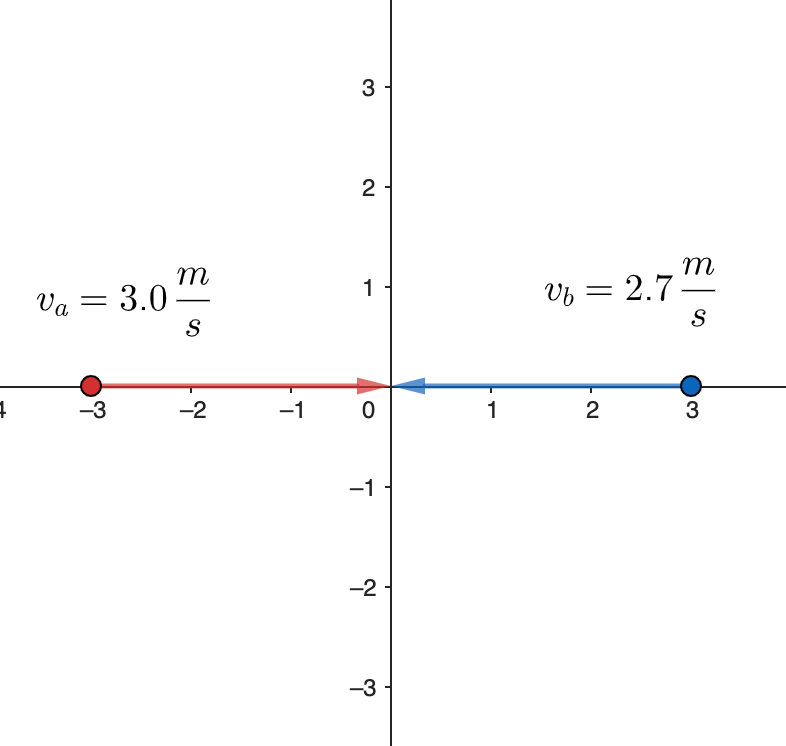
\includegraphics[scale=0.33]{./images/elastic_collision}
\end{minipage}
\begin{minipage}{0.5\textwidth}
    \begin{itemize}
        \item $m_{a} = 1.2g$
        \item $m_{b} = 1.3kg$
        \item $v_{a} = 3.0\frac{m}{s}$
        \item $v_{b} = 2.7\frac{m}{s}$
        \item $v_{a}\prime = ?$
        \item $v_{b}\prime = ?$
    \end{itemize}
\end{minipage}
\subsection*{7.3\hspace*{0.5cm}Elastic Momentum - Solve}
Because of the law of conservation of momentum this equation is Elastic. The kinetic energy of the objects will be same as they were before the collision.\newline\newline
\textbf{1.} $P_{tot} = P_{tot}\prime$ \\
\begin{adjustwidth}{0.6cm}{0pt}
    $(\cancel{m_{a}})({v}_{a}) + (\cancel{m_{b}})({v}_{b}) = (\cancel{m_{a}})({v}_{a})\prime + (\cancel{m_{b}})({v}_{b})\prime$ \\\\
    $({v}_{a}) + ({v}_{b}) = ({v}_{a})\prime + ({v}_{b})\prime$ \\\\
    $\therefore v_{a}\prime = v_{a} = 3.0\frac{m}{s}$ \\\\
    $\therefore v_{b}\prime = v_{b} = 2.7\frac{m}{s}$
\end{adjustwidth}\vspace*{15pt}
\textbf{2.} Proof of Elastic with $E_{tot} = E_{tot}\prime$ \\
\begin{adjustwidth}{0.6cm}{0pt}
    $\frac{1}{2}mv_{a} + \frac{1}{2}mv_{b} = \frac{1}{2}mv_{a}\prime + \frac{1}{2}mv_{b}\prime$ \\\\
    $\frac{1}{2}(1.2)(3.0) + \frac{1}{2}(1.3)(2.7) = \frac{1}{2}(1.2)(3.0) + \frac{1}{2}(1.3)(2.7)$ \\\\
    $\therefore$ Elastic $3.055 = 3.055$
\end{adjustwidth}\vspace*{15pt}